\documentclass[xcolor=table]{beamer}
\usepackage{array}
\usetheme{Berlin}
\usecolortheme{seahorse}
\usepackage[utf8]{inputenc}
\usepackage{color,xcolor,german, graphicx, listings, ifthen}
\definecolor{lightblue}{RGB}{230, 230, 250}
\setbeamerfont{frametitle}{size=\large}
\setbeamercovered{transparent}
\beamertemplatenavigationsymbolsempty
\setbeamertemplate{footline}[frame number]
\useoutertheme[width=60pt,height=25pt,right]{sidebar}
\lstdefinestyle{custom}{
  belowcaptionskip=1\baselineskip,
  breaklines=true,
  xleftmargin=\parindent,
  language=Java,
  showstringspaces=false,
  basicstyle=\tiny\ttfamily,
  keywordstyle=\tiny\bfseries\color{green!40!black},
  commentstyle=\tiny\color{purple!40!black},
  identifierstyle=\tiny\color{blue},
  stringstyle=\tiny\color{orange},
  backgroundcolor=\color{lightblue},
  escapeinside={\%*}{*)}
}
\lstset{style=custom}


\begin{document}

\newboolean{loesung}
\setboolean{loesung}{true}

\title{Software Engineering}
\author{Mark Keinh\"orster}
\institute{FOM \\ Hochschule f\"ur \"Okonomie und Management}
\date{\today}
\logo{
\includegraphics[scale=0.35]{FOMLogo.pdf}}
\begin{frame}
\titlepage
\end{frame}


\begin{frame}
	\frametitle{Inhaltsverzeichnis}
	\tableofcontents[hideallsubsections]
\end{frame}

%\part{Einfuehrung}

%----------------------------------------------------------------------------
\section{Vorraussetzungen}
\begin{frame}[fragile]
	\frametitle{Vorraussetzungen}
\huge Vorraussetzungen
\end{frame}

\begin{frame}
\frametitle{Ihre Erwartungen an die Veranstaltung}
	\begin{exampleblock}{Was m\"ochten Sie gerne behandeln?}
		\begin{itemize}
			 \item{}
			 \item{}
			 \item{}
			 \item{}
			 \item{}
		\end{itemize}
	\end{exampleblock}
\end{frame}

\begin{frame}
\frametitle{Erwartungen an die Veranstaltung}
	\begin{block}{Was sollten Sie am Ende k\"onnen?}
		\begin{itemize}
			 \item{Software Engineering als Teildisziplin der Informatik kennen}
			 \item{Grundpfeiler des Software Engineering kennen}
			 \item{Vorgehensmodelle der Softwareentwicklung beschreiben und abgrenzen}
			 \item{Softwarequalität messen und bewerten}
			 \item{Weiterf\"uhrende Konzepte verstehen und anwenden}
		\end{itemize}
	\end{block}
\end{frame}

%----------------------------------------------------------------------------
\section{Einführung}
\begin{frame}[fragile]
	\frametitle{Einführung}
\huge Einführung
\end{frame}

\begin{frame}[fragile]
	\frametitle{SW-Entwicklung im Studium}
	\begin{columns}
		\begin{column}{.5\textwidth}
			Aufgabe: Rekursives Take
			\newline\newline
			Implementieren Sie die Methode take(int n) die
			die ersten n Elemente eines Übergebenen Arrays
			vom Typ int als neues Array zurückgibt.
		\end{column}
		\begin{column}{.5\textwidth}
			\center
\includegraphics[width=1\textwidth,
			keepaspectratio=true]{bilder/student.png}
		\end{column}
	\end{columns}
\end{frame}

\begin{frame}
\frametitle{Die Realität}
	\begin{columns}
		\begin{column}{0.5\textwidth}
			\small
			\begin{itemize}
				\item Anforderungen mehrere 100 Seiten lang
				\item Anforderungen unklar, widersprüchlich, flexibel
				\item International verteilte Teams
				\item Mehrere tausend Nutzer in 5 Ländern
				\item Unterstützung von Chrome, Firefox, IE 6
				\item 6 Monate Projektlaufzeit, 500.000 LOC
			\end{itemize}
			\normalsize
		\end{column}
		\begin{column}{.5\textwidth}
			\center
\includegraphics[width=1\textwidth,
			keepaspectratio=true]{bilder/student_traurig.png}
		\end{column}
	\end{columns}
\end{frame}

\begin{frame}
\frametitle{Die Realität}
	Standish Group (http://www.standishgroup.com) veröffentlicht
	jährlich ``Chaos Report''.
	\newline\newline
	\begin{block}{Chaos Report 2015}
		\begin{itemize}
			\item 19\% der betrachteten IT-Projekte scheitern
			\item 52\% der betrachteten IT-Projekte drohen zu scheitern
			\item 29\% der betrachteten IT-Projekte sind erfolgreich
		\end{itemize}
	\end{block}
\end{frame}

\begin{frame}
\frametitle{Softwarekatastrophe ARIANE 5}
	\begin{quote}
		On June 4, 1996, on its maiden flight, the Ariane-5 was launched
		and performed perfectly for approximately 40 seconds. Then it began
		to veer off course. At the direction of the Ariane ground controller,
		the rocket was destroyed by remote control. \ldots total cost of the
		disaster was 500 million dollar.
	\end{quote}
	\begin{itemize}
		\item Flugbahn wird durch ``Inertial Reference System (SRI)'' gemessen,
		dessen Software teilweise von Ariane-4 übernommen wurde.
		\item Andere Flugbahndaten erzeugten Überlauf bei
		Konvertierung von 64-Bit Floating Point in 16-Bit Integer
		und verursachten Fehlfunktion des SRI-Systems.
	\end{itemize}
\end{frame}

\begin{frame}
\frametitle{Softwarekatastrophe Heartbleed}
	\begin{itemize}
		\item Heartbeat hält TLS-Verbindung am Leben
		\item Eine Seite schickt beliebig langen Payload, Gegenseite schickt die
		gleichen Daten wieder zurück
		\item Indikator für aufrechte Verbindung
	\end{itemize}
\end{frame}

\begin{frame}
\frametitle{Softwarekatastrophe Heartbleed}
	\center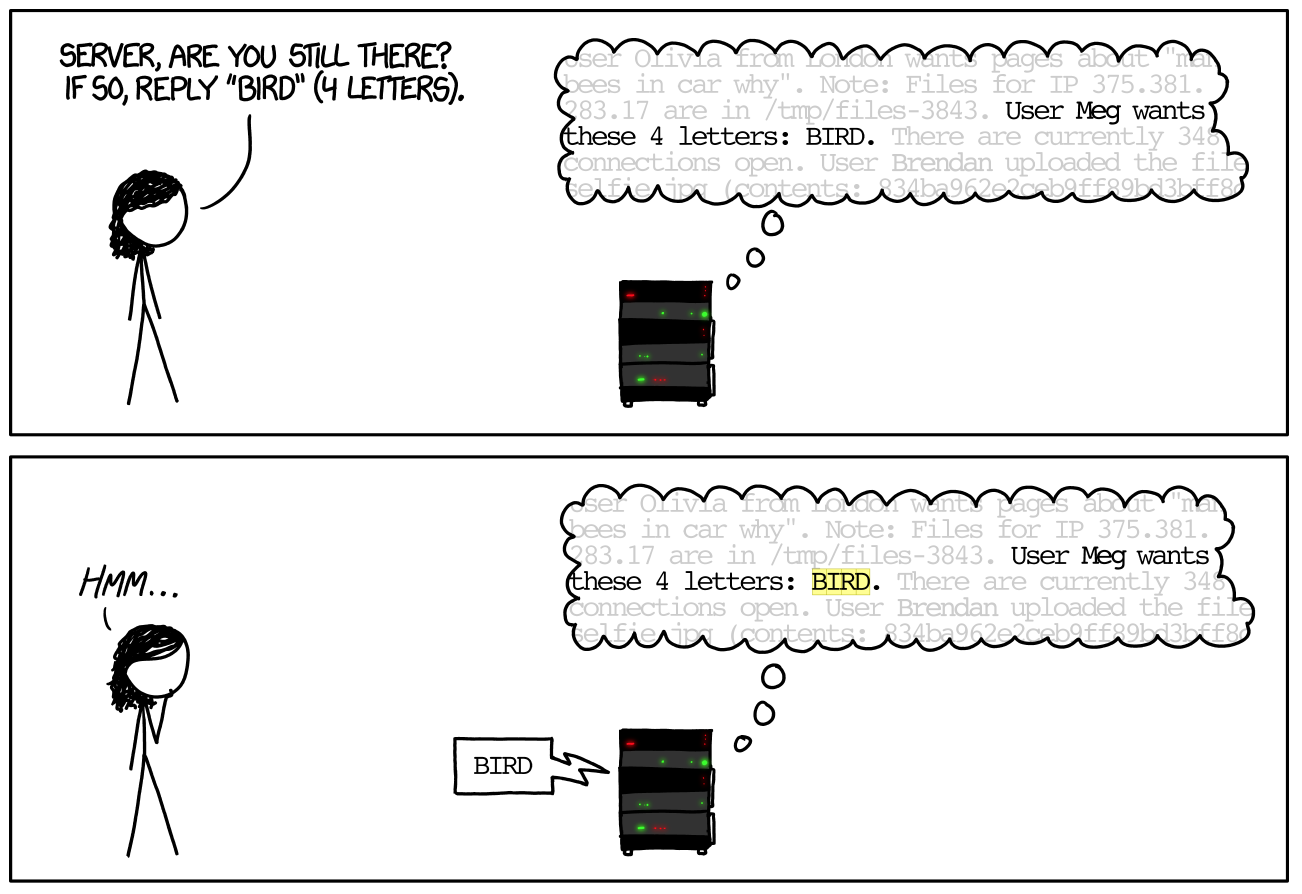
\includegraphics[width=1\textwidth,
	keepaspectratio=true]{bilder/heartbleed1.png}
\end{frame}

\begin{frame}
\frametitle{Softwarekatastrophe Heartbleed}
	\begin{itemize}
		\item Prüfung ob Payload der angegebenen Länge entspricht fehlte
		\item War der Payload kürzer als angegeben wurden Daten aus den darauffolgenden
		Speicherbereichen kopiert
		\item Da OpenSSL eine eigenen Speicherverwaltung implementiert waren diese Daten
		auch aus dem OpenSSL Kontext
	\end{itemize}
\end{frame}

\begin{frame}
\frametitle{Softwarekatastrophe Heartbleed}
	\center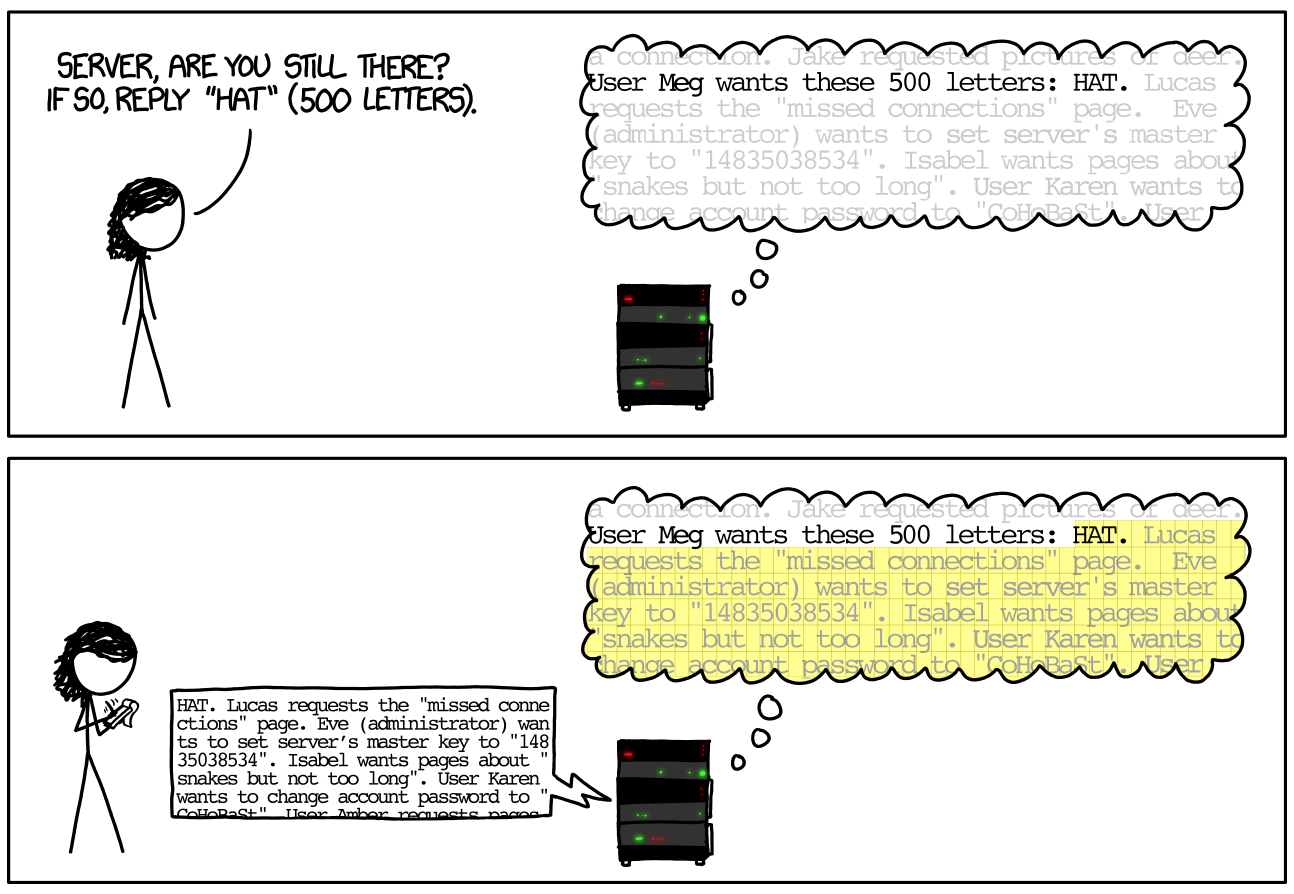
\includegraphics[width=1\textwidth,
	keepaspectratio=true]{bilder/heartbleed2.png}
\end{frame}

\begin{frame}
\frametitle{Softwarekrise}
	SW-Entwicklung in den 40er und 50er Jahren
	\small
	\begin{itemize}
		\item Teure Hardware
		\item Low-Level Programmierung (Assembler, fast kein OS)
		\item Von Experten bedient (Entwickler = Nutzer)
		\item numerisch-naturwissenschaftliche Probleme
	  	\item Codierung bekannter, mathematisch fundierter Algorithmen
	 	\item Viele Daten, einfache Algorithmen
		\item Häufig Batch-Systeme
		\item Fokus auf Effizienz
		\item Häufig ``Wegwerf-Software''
	\end{itemize}
	\normalsize
\end{frame}

\begin{frame}
\frametitle{Softwarekrise}
	SW-Entwicklung in den 60er Jahren bis heute
	\small
	\begin{itemize}
		\item Preiswerte Hardware mit viel Leistung
		\item Embedded Hardware die günstig ist und häufig eingesetzt wird
		\item Nicht-Informatiker nutzen die Software
		\item Vielzahl von Anwendungsbereichen
	  	\item Kritische Anwendungsbereiche wie Finanzsektor etc.
	  	\item Systeme sind komplex und interaktiv
		\item Software teurer als Hardware
		\item Lange Lebensdauer
	\end{itemize}
	\normalsize
\end{frame}

\begin{frame}
\frametitle{Softwarekrise}
	\begin{block}{Softwarekrise}
		\begin{itemize}
			 \item Programme werden immer komplexer
			 \item Passende Programmiersprachen, Methoden, Werkzeuge fehlen
		\end{itemize}
	\end{block}
	\begin{alertblock}{Folgen}
		\begin{itemize}
			 \item Kosten für Software steigen
			 \item Softwareprojekte scheitern
		\end{itemize}
	\end{alertblock}
	\begin{exampleblock}{Lösungsansatz}
		SW-Entwicklung als Ingenieurstätigkeit mit definiertem Vorgehen
		statt künstlerischer Tätigkeit
	\end{exampleblock}
\end{frame}

\begin{frame}
\frametitle{Softwarekrise}
	\begin{block}{Djikstra (The Humble Programmer)}
		\begin{quote}
			Als es noch keine Rechner gab, war auch das Programmieren noch kein
			Problem, als es ein paar leistungsschwache Rechner gab, war das
			Programmieren ein kleines Problem und nun, wo wir gigantische Rechner
			haben, ist das Programmieren zu einem gigantischen Problem geworden.
			In diesem Sinne hat die elektronische Industrie kein einziges Problem
			gelöst, sondern nur neue geschaffen. Sie hat das Problem geschaffen,
			ihre Produkte zu nutzen.
		\end{quote}
	\end{block}
\end{frame}

\begin{frame}
\frametitle{Was ist Software}
	\begin{block}{IEEE Definition}
		Software ist eine Sammlung von Computerprogrammen, Prozeduren, Regeln,
		zugehöriger Dokumentation und Daten
		\begin{itemize}
			 \item Programme sind eine Teilmenge von Software
			 \item SW beeinhaltet Dokumente die verschiedene Abstraktionsschichten
			 für verschiedene Zielgruppen beschreiben
		\end{itemize}
	\end{block}
\end{frame}

\begin{frame}
\frametitle{Probleme bei der Softwareentwicklung}
	\begin{itemize}
		 \item Kommunikationsprobleme mit Anwender
		 \item SW ist immateriell
		 \item SW ist leicht modifizierbar, Behebung von Fehlern wird unterschätzt
		 \item SW ist nur beobachtbar
		 \item Anforderungen ändern sich regelmäßig
		 \item SW altert über Umgebung ohne zu Verschleißen,
		 das führt zu immer neuen Erweiterungen und wachsender Komplexität
		 \item Verhalten für Software lässt sich nur schwer beweisen
		 \item \ldots
	\end{itemize}
\end{frame}

\begin{frame}
\frametitle{Software Engineering}
	\begin{itemize}
		\item Auslöser für Begriff ``Software Engineering'' war Softwarekrise von 1968
		\item Begriff ``Software Engineering'' wurde 1967 von F.L. Bauer (ehemaliger Prof. in München) 
		im Rahmen einer ``Study Group on Computer Science'' der NATO geprägt.
		\item Software wurde erstmals als Industrieprodukt bezeichnet
	\end{itemize}
\end{frame}

\begin{frame}
\frametitle{Was ist Software Engineering}
	\begin{block}{Definition IEEE}
		Software Engineering ist der systematische Ansatz für
		\begin{itemize}
			\item die Entwicklung,
			\item den Betrieb
			\item sowie die Wartung
		\end{itemize}
		von Software.
	\end{block}
\end{frame}

\begin{frame}
\frametitle{Was ist Software Engineering}
	\begin{block}{Definition Lehrbuch Software-Technick (Balzert) }
		Zielorientierte Bereitstellung und systematische Verwendung von Prinzipien, Methoden, Konzepten, 
		Notationen und Werkzeugen für die arbeitsteilige, ingenieurmäßige Entwicklung und Anwendung von 
		umfangreichen Software-Systemen. Zielorientiert bedeutet die Berücksichtigung z.B. von Kosten, 
		Zeit, Qualität.
	\end{block}
\end{frame}

\begin{frame}
\frametitle{Ziele des Software Engineerings}
	Effiziente Entwicklung von messbar qualitativ hochwertiger Software
	\small
	\begin{itemize}
		\item Korrektheit und Zuverlässigkeit
		\item Robustheit
		\item Effizienz
		\item Benutzerfreundlichkeit
		\item Wartbarkeit und Wiederverwendbarkeit
	\end{itemize}
	\normalsize
	Qualitätsfaktoren
	\small
	\begin{itemize}
		\item Extern (für den Benutzer sichtbar)
		\item Intern (nur für den Entwickler sichtbar)
	\end{itemize}
	\normalsize
	\normalsize
\end{frame}

\begin{frame}
\frametitle{Phasen des Software Engineering}
Der systematische Ansatz im Software Engineering wird auch als
Entwicklungsprozess bezeichnet. Er beeinhaltet eine Reihe von Aktivitäten
die zur Entwicklung von Software führen.
\begin{itemize}
	\item Spezifikation
	\item Entwicklung
		\begin{itemize}
			\item Entwurf
			\item Implementierung
		\end{itemize}
	\item Validierung
	\item Evolution
		\begin{itemize}
			\item Weiterentwicklung
			\item Betrieb
		\end{itemize}
\end{itemize}
\end{frame}

\begin{frame}
\frametitle{Kleine Softwareprojekte}
	\begin{itemize}
		\item Wenige LOC
		\item SW für die eigene Verwendung
		\item Produkt spezifiziert sich selbst
		\item Lösung wird direkt entwickelt
		\item Validierung und Korrekturen am Endprodukt
		\item 1 Entwickler
		\item Komplexität gering
		\item Software besteht aus wenigen Komponenten
		\item Wenig bis keine Dokumentation nötig
		\item Keine Planung und Projektstruktur nötig
	\end{itemize}
\end{frame}

\begin{frame}
\frametitle{Große Softwareprojekte}
	\begin{itemize}
		\item Viele LOC
		\item SW für die Verwendung durch Dritte
		\item Klares Ziel, genaue Spezifikation erforderlich
		\item Lösung wird in Phasen entwickelt
		\item Tests in jeder Phase sind unerlässlich
		\item Produkt wird im Team entwickelt
		\item Hohe Komplexität macht Strukturierung der SW erforderlich
		\item Software besteht aus vielen Komponenten
		\item Dokumentation für den wirtschaftlichen Betrieb der SW erfoderlich
		\item Projektstruktur zwingend erforderlich
	\end{itemize}
\end{frame}

\begin{frame}
\frametitle{Wachstum des Kommunikationsbedarfs}
	\center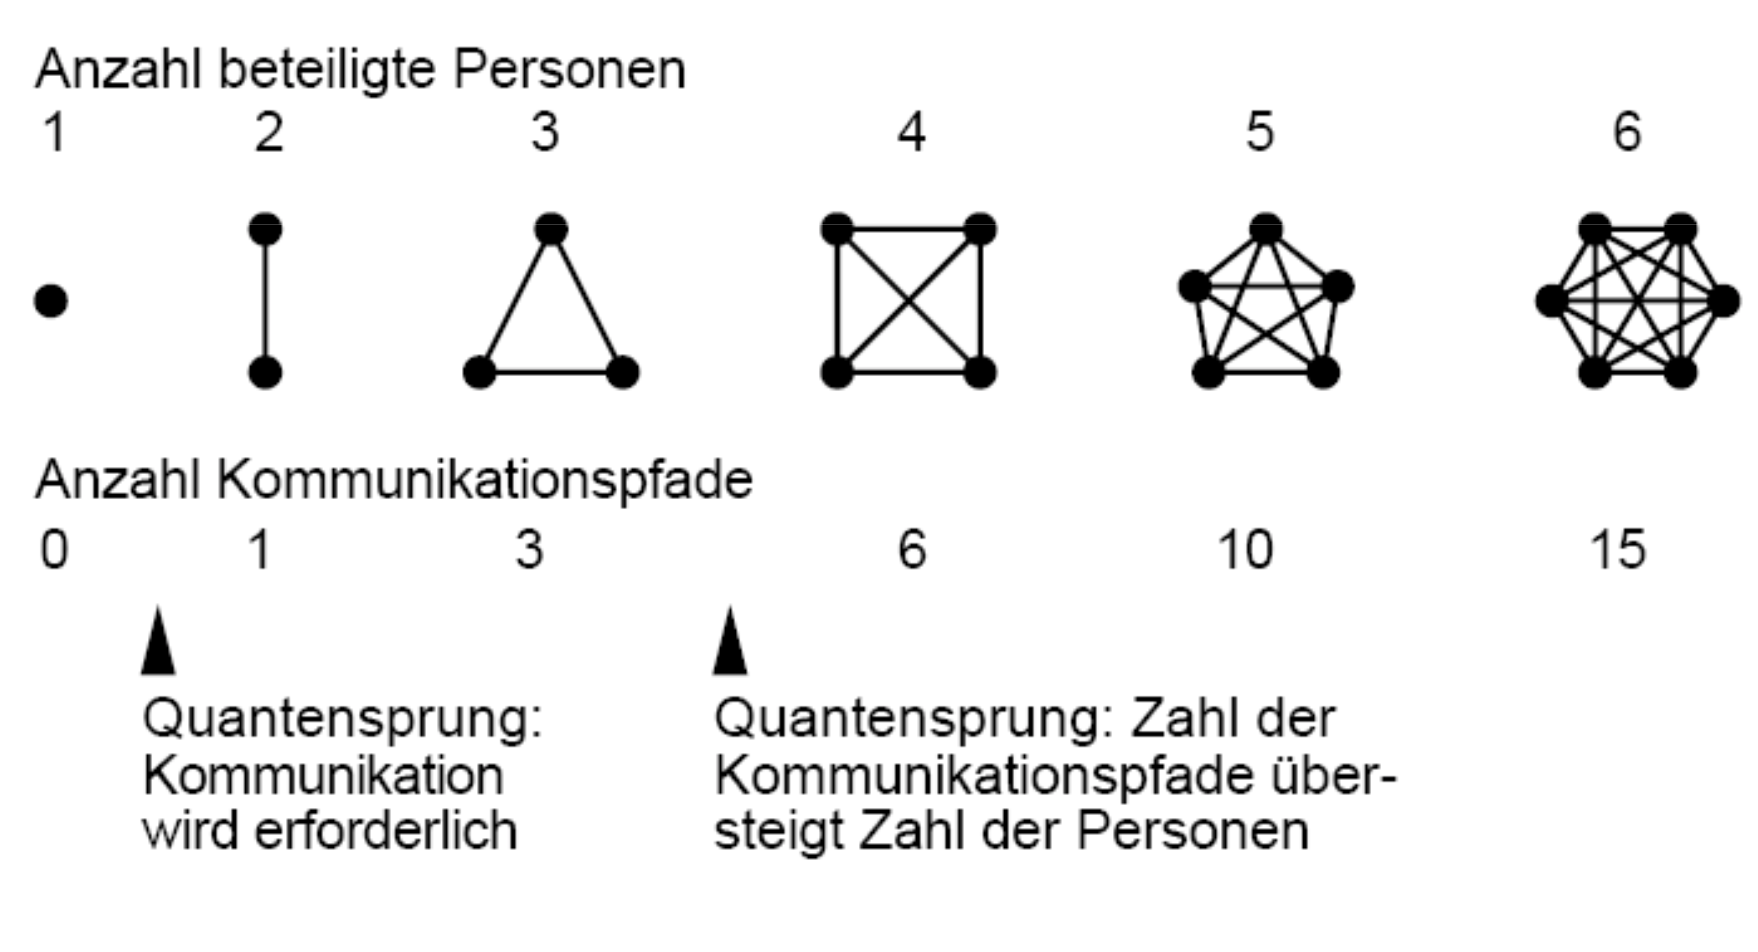
\includegraphics[width=1\textwidth,
	keepaspectratio=true]{bilder/kommunikationsbedarf.png}
\end{frame}

\begin{frame}
\frametitle{Wachstum des Aufwands}
	\center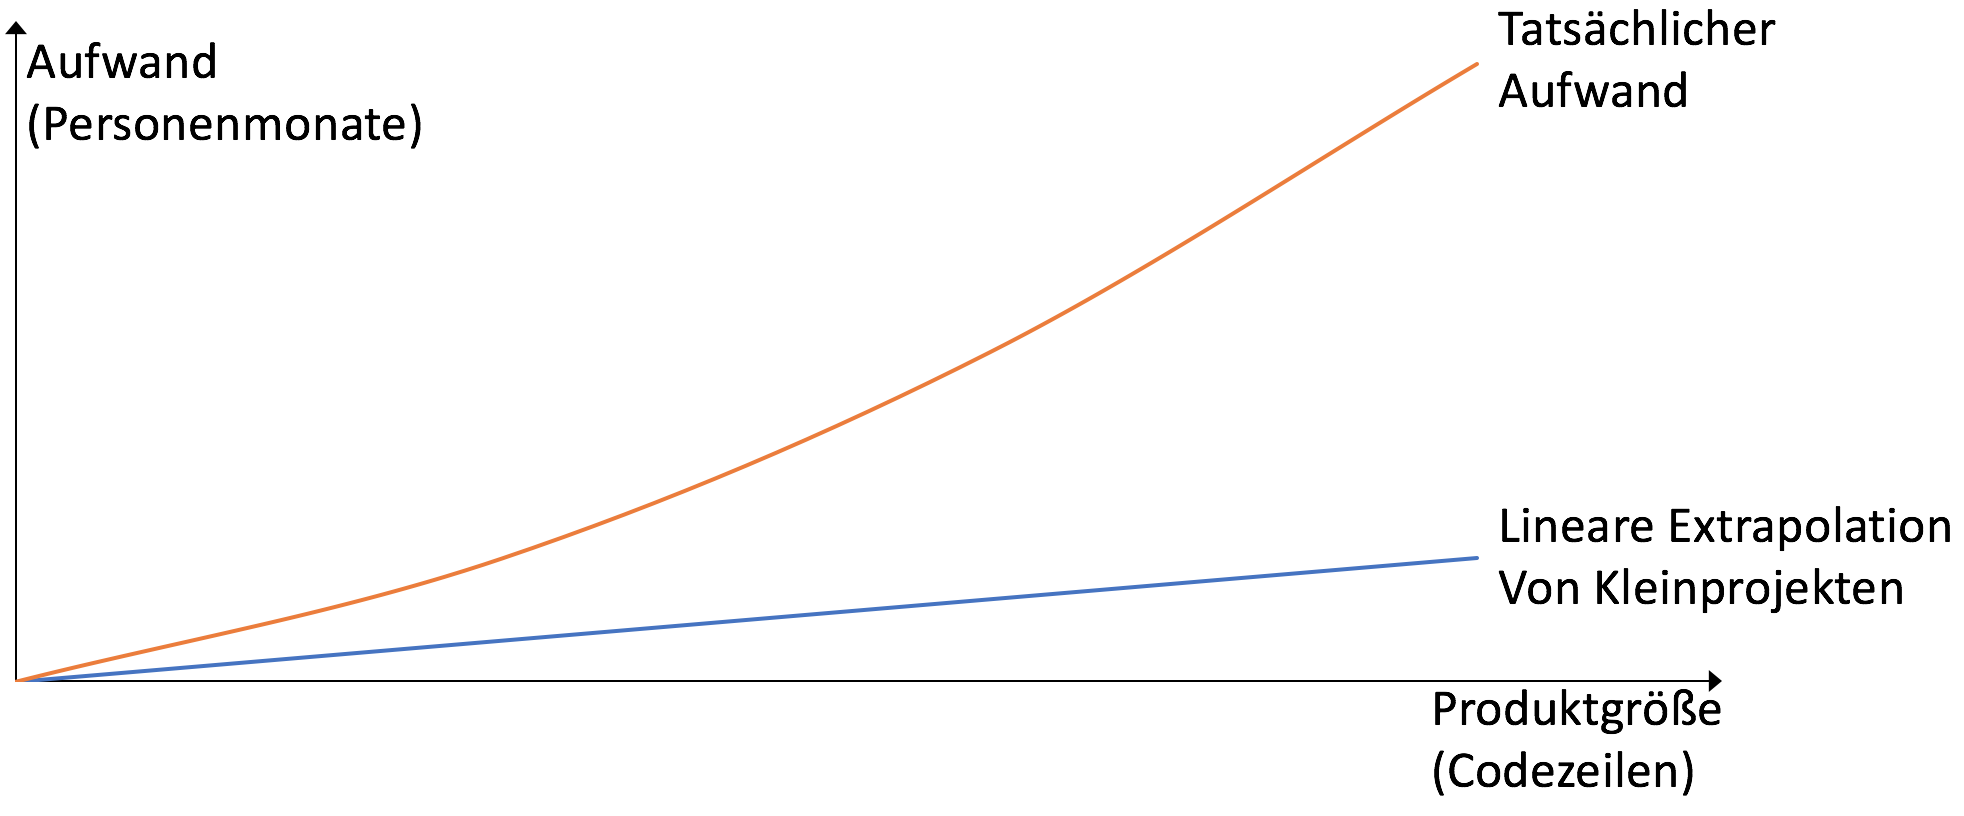
\includegraphics[width=1\textwidth,
	keepaspectratio=true]{bilder/projektaufwand.png}
\end{frame}

\begin{frame}
\frametitle{Aufwände aufgeschlüsselt}
	\center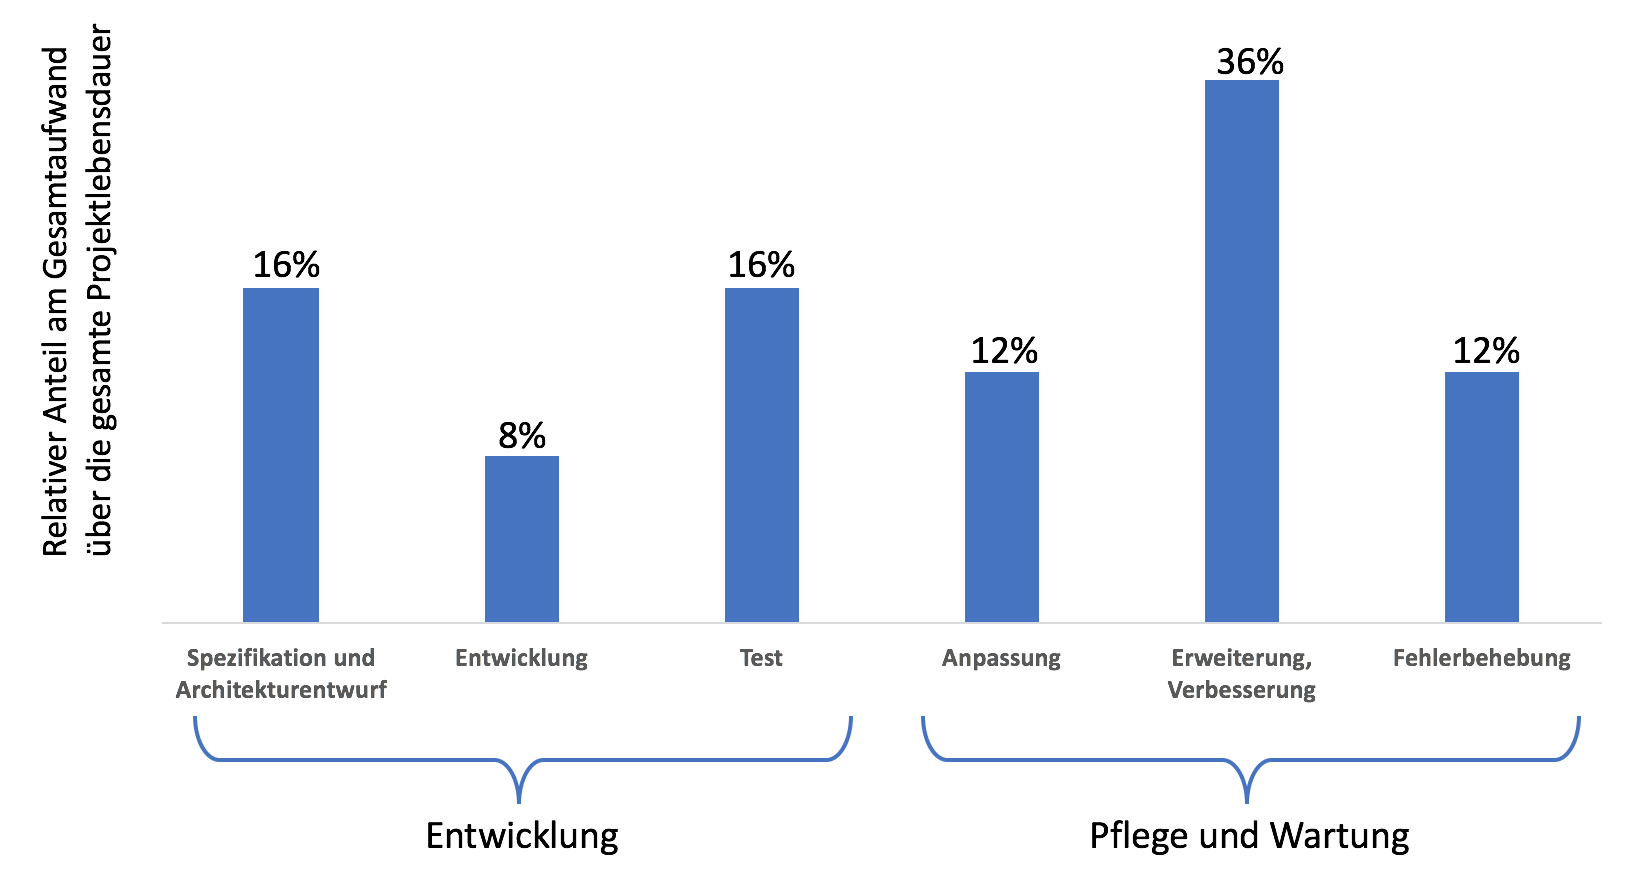
\includegraphics[width=1\textwidth,
	keepaspectratio=true]{bilder/anteil_aufwand.png}
\end{frame}

\begin{frame}
\frametitle{Übung 1.1}
	Eine Person braucht zum Bau einer 2m langen Bruecke 0,5 Tage. Wie lange brauchen 100 Leute für den Bau einer 2km langen Brücke?
	\begin{enumerate}
		\item Interpolieren Sie den Aufwand linear
		\item Warum ist die Berechnung aus Punkt 1 eine Milchmädchenrechnung?
	\end{enumerate}
\end{frame}

\begin{frame}
\frametitle{Übung 1.1 - Lösung}
	Eine Person braucht zum Bau einer 2m langen Bruecke 0,5 Tage. Wie lange brauchen 100 Leute für den Bau einer 2km langen Brücke?
	\begin{enumerate}
		\item Aufwand = (2000m / 2m * 0.5PT) / 100 Personen = 5 Tage
		\item Mehr Kommunikation, Projekt deutlich Komplexer, Ressourcenbeschaffung, Logistik ...
	\end{enumerate}
\end{frame}

\begin{frame}
\frametitle{Übung 1.2}
	\scriptsize
	Eine Kundenbetreuerin im Firmenkundengeschäft einer Bank hat auf Grundlage eines 
	Tabellenkalkulationsprogramms eine kleine persönliche Anwendung geschrieben, 
	die sie bei der Überprüfung der Kredite der von ihr betreuten Firmen unterstützt. 
	Die notwendigen Daten gibt sie jeweils von Hand ein. Der Abteilungsleiter sieht 
	diese Anwendung zufällig, ist davon angetan und beschließt, sie allen Kundenbetreuerinnen 
	und -betreuer zur Verfügung stellen. Die notwendigen Daten sollen jetzt automatisch aus 
	den Datenbanken der Bank übernommen werden. Die Kundenbetreuerin gibt an, für die Entwicklung 
	ihrer Anwendung insgesamt etwa vier Arbeitstage aufgewendet zu haben. Der Abteilungsleiter 
	veranschlagt daher für die Übernahme und die gewünschten Änderungen einen Aufwand von einer 
	Arbeitswoche. Als die geänderte Anwendung endlich zur Zufriedenheit aller Beteiligten läuft, 
	sind jedoch rund acht Arbeitswochen Aufwand investiert. Der Abteilungsleiter erzählt die 
	Geschichte einem befreundeten Berater als Beispiel, dass Informatikprojekte nie ihre Termine 
	einhalten. Darauf meint der Berater trocken, der investierte Aufwand sei völlig realistisch 
	und normal. Begründen Sie warum.
	\normalsize
\end{frame}

\begin{frame}
\frametitle{Übung 1.2 - Lösung}
	\scriptsize
	\begin{itemize}
		\item Die Kundenbetreuerin hat das Fachkonzept ihrer Tabellenkalkulationsanwendung vermutlich 
		schon vor den angegebenen vier Tagen Bearbeitungszeit im Kopf gehabt. Die Fremdentwickler 
		müssen dieses zumindest erst nachvollziehen.
		\item Die neue Anwendung ist durch die Datenbankanbindung mit den entsprechenden Schnittstellen 
		und Zugriffsrechteproblematiken deutlich komplexer.
		\item Der Kommunikationsaufwand schon allein von Kundenseite (viele Berater = viele unterschiedliche 
		Meinungen) ist erheblich
		\item Die neu entstandene ``professionelle'' Anwendung hat einen erheblich höheren Aufwand für 
		die Validierung als eine eigengenutzte Entwicklung.
		\item An die Bedienbarkeit (Nutzerschnittstelle) werden bei einer ``professionellen'' Anwendung 
		erheblich höhere Ansprüche gestellt.
	\end{itemize}
\end{frame}

\section{Vorgehensmodelle}
\begin{frame}[fragile]
\frametitle{Vorgehensmodelle}
\huge Vorgehensmodelle
\end{frame}

\begin{frame}
\frametitle{Begriffe}
	\begin{block}{Definition ``Prozess'' nach IEEE}
		Eine Folge von Schritten die zu einem definierten Zweck ausgeführt werden
		\begin{itemize}
			\item Beispielsweise der Softwareentwicklungsprozess
			\item Um Operationen auf Daten auszuführen
		\end{itemize}
		von Software.
	\end{block}	
\end{frame}

\begin{frame}
\frametitle{Begriffe}
	\begin{block}{Definition ``Softwareentwicklungsprozess'' nach IEEE}
		Der Prozess bei dem die Bedürfnisse von Nutzern in ein Softwareprodukt übersetzt werden.
		Der Prozess beeinhaltet
		\begin{itemize}
			\item das Übersetzen der Bedürfnisse in konkrete Anforderungen,
			\item die Überführen der Anforderungen in einen Entwurf,
			\item die Implementierung des Entwurfs in Quelltext,
			\item das Testen des Quelltextes,
			\item die Installation und den Betrieg der implementierten Software.
		\end{itemize}
	\end{block}	
\end{frame}

\begin{frame}
\frametitle{Softwareentwicklungsprozesse in der Praxis}
\begin{itemize}
	\item Softwareprozesse variieren je nach Organisation
	\item kein Prozess ist perfekt
	\item Folge: Ergebnisse unterscheiden sich situationsbedingt
\end{itemize}
\end{frame}

\begin{frame}
\frametitle{Übung 2.1}
	Geben Sie
	\begin{enumerate}
		\item Beispiele für unterschiedliche Softwareprozesse
		\item Gründe für diese Unterschiede
	\end{enumerate}
	Warum ist es schwierig Softwareentwicklungsprozesse zu automatisieren?
\end{frame}

\ifloesung
\begin{frame}
\frametitle{Übung 2.1 - Lösung}
	\scriptsize
	Beispiele für unterschiedliche Softwareprozesse
	\begin{enumerate}
		\item Planungsgetriebene Prozesse
		\begin{itemize}
			\item Sequenziell
			\item Nebenläufig
			\item Inkrementell
		\end{itemize}
		\item Agile Prozesse
		\item \ldots
	\end{enumerate}
	\bigskip
	Gründe für diese Unterschiede
	\begin{enumerate}
		\item Detailgrad der Anforderungen
		\item Teamstruktur
		\item Planbarkeit des Softwareprodukts
		\item Time-2-Market
		\item Art der Software die Entwickelt wird
		\item Kundentyp
		\item \ldots
	\end{enumerate}
	\normalsize
\end{frame}

\begin{frame}
\frametitle{Übung 2.1 - Lösung}
	\scriptsize
	Warum ist es schwierig Softwareentwicklungsprozesse zu automatisieren?
	\begin{enumerate}
		\item Anforderungen oft nicht final
		\item Komplexe Systeme sehr schwer zu testen
		\item Große Systeme besitzen viele Schnittstellen
		\item \ldots
	\end{enumerate}
	\normalsize
\end{frame}
\fi

\begin{frame}
\frametitle{Prozessmodell vs konkreter Prozess}
	Modell
		\begin{itemize}
			\item Abstrakte Abfolge von Schritten
			\item Dient beliebig vielen Prozessen als Grundlage für konkretes Vorgehen
			\item Ist ein Muster für eine bestimmte Vorgehensweise
		\end{itemize}
	\bigskip
	Prozess = Gegenstand des Modells
		\begin{itemize}
			\item Tatsächlich ausgeführte Abfolge von Schritten
			\item Jeder Schritt produziert konkretes Ergebniss
			\item Ist das Projekt
		\end{itemize}
\end{frame}

\begin{frame}
\frametitle{Beispiele Modell vs konkreter Gegenstand}
	\begin{columns}
		\begin{column}{0.5\textwidth}
		Modell
			\small
			\begin{itemize}
				\item Theaterstück
				\item Musik-CD
				\item Applikation
				\item Klasse
				\item Vorgehensmodell
				\item Prozessmodell
			\end{itemize}
			\normalsize
		\end{column}
		\begin{column}{.5\textwidth}
		Gegenstand
			\small
			\begin{itemize}
				\item Aufführung
				\item Einmalige Wiedergabe
				\item Ausführung der Applikation
				\item Objekt
				\item Projektablauf
				\item Projekt (inkl. Organisation)
			\end{itemize}
			\normalsize
		\end{column}
	\end{columns}
\end{frame}

\begin{frame}
\frametitle{Merkmale von Modellen}
	Abbildungsmerkmal
	\begin{itemize}
		\item Ein Modell ist immer ein Abbild des Originals
		\item dass 
		\begin{itemize}
			\item Struktur (z.B. Aufbau eines Hauses), 
			\item Verhalten (z.B. Schiffsmodell im Strömungskanal)
			\item oder Funktionsweise (z.B. Modellauto dass fährt)
		\end{itemize}
		des Originals abbildet.
	\end{itemize}
	\bigskip
	Verkürzungsmerkmal
	\begin{itemize}
		\item Es enthält die relevanten Eigenschaften wie
		\begin{itemize}
			\item detaillierter Skelettaufbau des Menschen für Ärzte
			\item oder die Beschreibung der Proportionen des Menschen für Schneider
		\end{itemize}
	\end{itemize}
	\bigskip
	Pragmatisches Merkmal
	\begin{itemize}
		\item Es ist zugeschnitten auf den Untersuchungszweck und kann damit
		unter bestimmten Bedingungen das Original ersetzen
	\end{itemize}
	\bigskip
\end{frame}

\begin{frame}
\frametitle{Modelle beim Software Engineering}
	Software wird auf unterschiedliche Arten repräsentiert (Software Modelle)
		\begin{itemize}
			\item Spezifikation
			\item Entwurf
			\item Diagramme
			\item Code
			\item Kennzahlen
			\item Dokumentation
		\end{itemize}
	\bigskip
	Abläufe bei der Entwicklung von Software werden durch Vorgehens-/Prozessmodelle beschrieben
\end{frame}

\subsection{Basismodelle}
\begin{frame}
\frametitle{Basismodelle}
\huge Basismodelle
\end{frame}

\begin{frame}
\frametitle{Basismodelle}
	\begin{block}{Definition Vorgehensmodell}
		Darstellung, die weitgehend den Softwareentwicklungsprozess beschreibt und prinzipiell 
		auch Analysen des Prozesses gestattet.
		Ein Vorgehensmodell muss die Prozessschritte und die dabei verwendeten und entwickelten 
		Resultate explizit beschreiben.
	\end{block}
\end{frame}

\begin{frame}
\frametitle{Code and Fix}
	
\end{frame}

\begin{frame}
\frametitle{Sequenzielles Modell}
	
\end{frame}

\begin{frame}
\frametitle{Wasserfallmodell als bekanntestes sequentielles Modell}
	
\end{frame}

\begin{frame}
\frametitle{Nebenläufiges Modell}
	
\end{frame}

\begin{frame}
\frametitle{Inkrementelles Modell}
	
\end{frame}

\begin{frame}
\frametitle{Evolutionäres Modell}
	
\end{frame}

\begin{frame}
\frametitle{Prototypen}
	
\end{frame}

\begin{frame}
\frametitle{Pilotsystem}
	
\end{frame}

\begin{frame}
\frametitle{Spiralmodell}
	
\end{frame}

\subsection{Monumentale Prozessmodelle}
\begin{frame}
\frametitle{Monumentale Prozessmodelle}
\huge Monumentale Prozessmodelle
\end{frame}

\begin{frame}
\frametitle{Monumentale Prozessmodelle}
	\begin{block}{Definition Prozessmodell}
		Während Vorgehensmodelle den Kern bilden, ergänzen Prozessmodelle die Vorgehensmodelle um 
		Organisationsstrukturen für Projektmanagement, Qualitätssicherung, Dokumentation sowie 
		Konfigurationsverwaltung.
	\end{block}
\end{frame}

\begin{frame}
\frametitle{Monumentale Prozessmodelle}
	\begin{itemize}
		\item Aktivitäten werden von Mitarbeitern durchgeführt
		\item Die Kenntnisse/Fähgikeiten die als Vorraussetzung dienen
		werden durch Rollen beschrieben
		\item Die Durchführung wird genauer spezifiziert
		\begin{itemize}
			\item Weitere durchzuführende Aktivität?
			\item Rollenzuordnung
			\item Zu verwendende Artifakte
			\item Zu erstellende Artifakte
			\item Zu beachtende Konventionen, Methoden, Richtlinien
			\item Einzusetzende Werkzeuge
		\end{itemize}
	\end{itemize}
\end{frame}

\begin{frame}
\frametitle{Monumentale Prozessmodelle}
	\center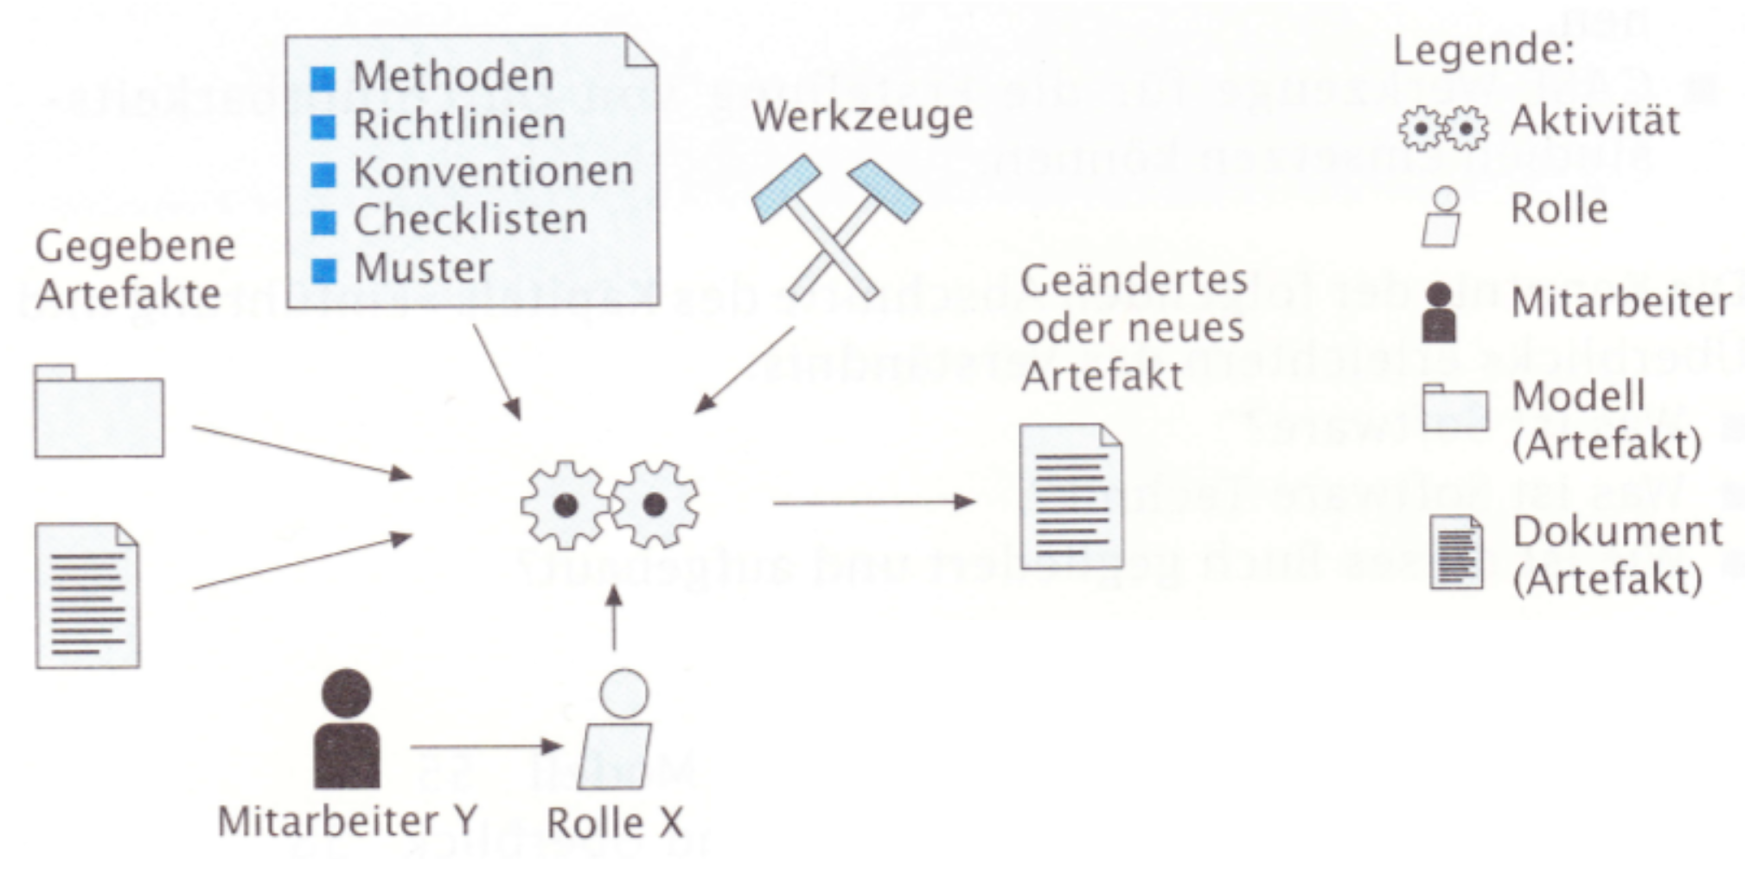
\includegraphics[width=1\textwidth,
			keepaspectratio=true]{bilder/prozessmodell.png}
\end{frame}

\begin{frame}
\frametitle{V-Modell}
	
\end{frame}

\begin{frame}
\frametitle{Rational Unified Process}
	
\end{frame}

\subsection{Agile Prozessmodelle}
\begin{frame}
\frametitle{Agile Prozessmodelle}
\huge Agile Prozessmodelle
\end{frame}

\begin{frame}
\frametitle{Agile Prozessmodelle}

\end{frame}

\begin{frame}
\frametitle{Extreme Programming}
	
\end{frame}

\begin{frame}
\frametitle{Scrum}
	
\end{frame}

\begin{frame}
\frametitle{Kanban}
	
\end{frame}


% ----------------------------------------------------------------------------
\section{Projektmanagement}
\begin{frame}[fragile]
	\frametitle{Projektmanagement}
\huge Projektmanagement
\end{frame}

\begin{frame}
\frametitle{Erfolgskriterien}
	Es gibt einige, allgemeine Erfolgskriterien die alle Projekte teilen
	\begin{itemize}
		\item Software wird innerhalb der definierten Zeit fertiggestellt
		\item Kosten liegen innerhalb der Budgetplanung
		\item Gelieferte Software entspricht der Erwartung des Kunden
		\item Entwicklungsteam arbeitet kohärent und effizient zusammen
	\end{itemize}
\end{frame}

\begin{frame}
\frametitle{Charakteristika von Softwareprojekten}
	Softwareprojekte haben bestimmte Charakteristika die sie von Projekten
	in anderen Bereichen unterscheiden
	\begin{itemize}
		\item Software ist intangibel
		\item Große SW-Projekte sind in Technologie, Vorgehen, Organisation
		einzigartig
		\item Prozesse und Vorgehensmodelle sind flexibel und organisationsspezifisch
	\end{itemize}
\end{frame}

\begin{frame}
\frametitle{Managementfaktoren in SW-Projekten}
	\begin{itemize}
		\item Größe der Organisation
		\item Kundentyp
		\item Komplexität der Software
		\item Softwaretyp
		\item Unternehmenskultur
		\item Softwareentwicklungsprozesse
	\end{itemize}
\end{frame}

\begin{frame}
\frametitle{Fundamentale PM Aktivitäten}
	\begin{enumerate}
		\item Projektplanung
		\item Risikomanagement
		\item Personalführung
		\item Berichterstattung
		\item Projektierung
	\end{enumerate}
\end{frame}

\subsection{Risikomanagement}
\begin{frame}
\frametitle{Risikomangement}
\huge Risikomangement
\end{frame}

\begin{frame}
\frametitle{Risikomanagement}
	\begin{block}{Risiko}
		Ein Problem, das noch nicht eingetreten ist, aber wichtige Projektziele
		oder Projektergebnisse gefährdet, falls es eintritt. Ob es eintreten wird
		kann nicht sicher vorausgesagt werden.
	\end{block}
	\begin{itemize}
		\item In jedem Projekt treten Probleme auf die die Projektziele gefährden
		\item Risikomanagement versucht mögliche Probleme frühzeitig zu identifizieren
		und Maßnahmen einzuleiten
		\item Risikomanagement ist eine kontinuierliche Aktivität und umfasst
		\begin{itemize}
			\item Identifikation von Risiken
			\item Analyse und Bewertung der Risiken
			\item Planung von Gegenmaßnahmen
			\item Risikoüberwachung
		\end{itemize}
	\end{itemize}
\end{frame}

\begin{frame}
\frametitle{Identifikation von Risiken}
	Eine Risikoeinordnung kann sein
	\begin{itemize}
		\item Projektrisiken die den Projektplan oder -ressourcen beeinflussen
		\item Produktrisiken die Qualität oder Effizienz der Applikation mindern
		\item Geschäftsrisiken den zugrundeliegenden Business Plan der Applikation beeinflussen
	\end{itemize}
\end{frame}

\begin{frame}
\frametitle{Identifikation von Risiken}
	\begin{itemize}
		\item Es kann auch zwischen Kernrisiken und projektspezifischen Risiken unterschieden werden.
		\item Projektspezifischre Risiken können beispielsweise im Rahmen eines moderierten
		Workshops erhoben werden
	\end{itemize}
\end{frame}

\begin{frame}
\frametitle{Übung 3.1}
	Überlegen Sie, welche Kernrisiken für einen Großteil der Soll-Ist-Abweichungen
	in Softwareprojekten verantwortlich ist.
\end{frame}

\ifloesung
\begin{frame}
\frametitle{Übung 3.1 - Lösung}
	\begin{itemize}
		\item Unklare bzw. sich laufend ändernde Projektziele und Anforderungen
					die grundlegende Änderungen am Quellcode erfordern
		\item Unkorrekter Zeitpland, z.B. die
					Dauer der Testphase wurde unterschätzt oder gar unterschlagen
		\item Mitarbeiterfluktuation im Projektteam
		\item Mangelnde Skills der Mitarbeiter
		\item Fehlende Unterstützung im Management
		\item Organisatorische Änderungen wie beispielsweise wechselnde Projektverantwortliche
		\item Grundlegend falsch gewählte Technologien
		\item \ldots
	\end{itemize}
\end{frame}
\fi

\begin{frame}
\frametitle{Analyse und Bewertung von Risiken}
	\begin{block}{Risikowert}
		Risikowert = p * K
		\begin{itemize}
			\item p = Eintrittswahrscheinlichkeit
			\item K = Kosten die im Schadensfall enstehen
		\end{itemize}
	\end{block}
	\begin{itemize}
		\item Risiken mit p \textgreater 0.5 sollten als sicheres Ereignis angesehen werden
		\item Jeder Risikowert kann als Punkt in einem Risikodiagramm eingesetzt werden
		\item Ein Risikodiagramm besitzt auf beiden Achsen eine logarithmische Skalierung
		\item Kleine Risikowerte müssen nicht Kontrolliert werden
	\end{itemize}
\end{frame}

\begin{frame}
\frametitle{Risikodiagramm}
	Das dargestellte Risikodiagramm bewertet Risikowerte bis 10000 Euro als akzeptabel
	\center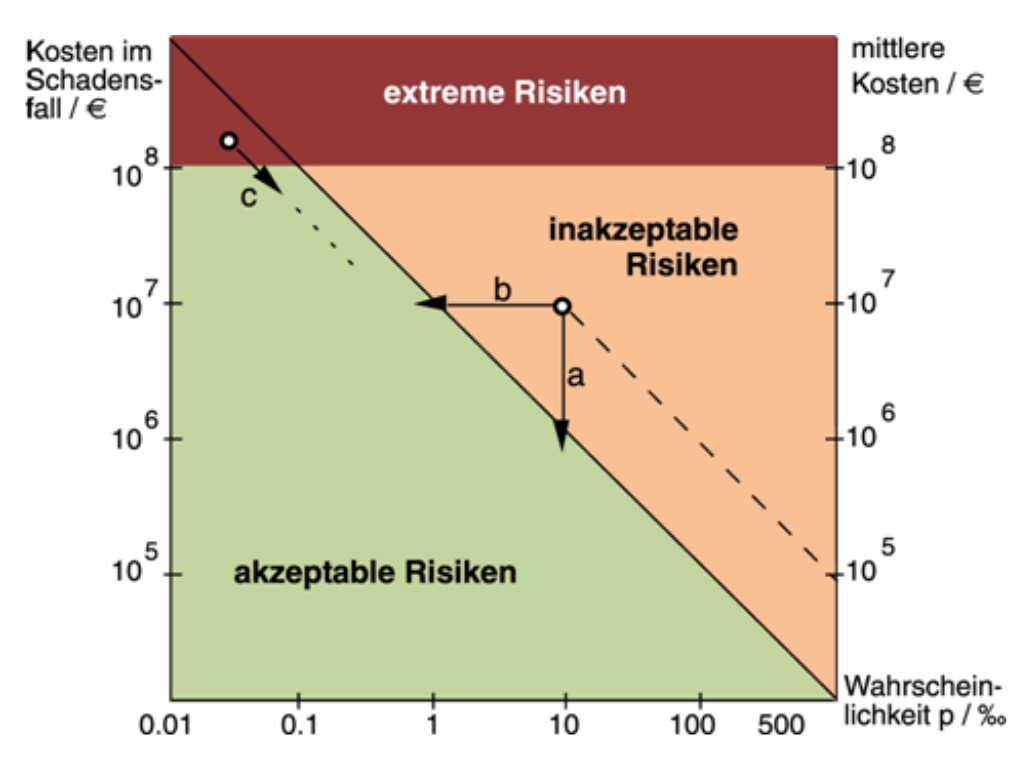
\includegraphics[width=1\textwidth,
		keepaspectratio=true]{bilder/risikodiagramm.png}
\end{frame}

\begin{frame}
\frametitle{Risikodiagramm}
	\begin{itemize}
		\item Für Punkte unter der Diagonalen sind keine Aktionen erforderlich
		\item Punkte über der Diagonalen müssen nach links oder unten verschoben werden
		\item Senkung der Kosten bei Risikoeintritt verschiebt den Punkt nach unten (Pfeil a)
		\item Senkung der Wahrscheinlichkeit verschiebt den Punkt nach links (Pfeil b)
		\item Alle Maßnahmen führen zu zusätzlichen sicheren Kosten die deutlich geringer sind
					als der mögliche Schaden
		\item Oben liegen extreme Risiken deren Schaden nicht beherrschbar ist (z.B. Firmenbankrott)
		\item Bei einem solchen Extremrisiko kann eine Versicherung in Erwägung gezogen werden die aus
					großem Eintrittschaden eine kleinere sichere Zahlung macht (Pfeil c)
	\end{itemize}
\end{frame}

\begin{frame}
\frametitle{Risikomatrix}
	Alternativ kann man mit einer diskreten Bewertung arbeiten
		\begin{table}[]
			\begin{tabular}{ll}
			 Wert (p) & Eintrittswahrscheinlichkeit \\
			 \hline
			 1 & Unwahrscheinlich \\
			 2 & Denkbar \\
			 3 & Wahrscheinlich \\
			 	 &	\\
			 Wert (k) & Schadensausmaß \\
			 \hline
			 1 & Gering \\
			 2 & Beträchtlich \\
			 3 & Groß
			\end{tabular}
		\end{table}
\end{frame}

\begin{frame}
\frametitle{Risikomatrix}
	Die Risiken können entsprechend klassifiziert werden um daraus eine Risikomatrix
	abzuleiten.
	\bigskip
	\begin{small}
		\begin{table}[]
			\begin{tabular}{l|lll}
			 Groß 				& \cellcolor[HTML]{FFCD69} 3 & \cellcolor[HTML]{FC6D58} 6 & \cellcolor[HTML]{D8334A} 9 \\
			 Beträchtlich & \cellcolor[HTML]{E8CE4D} 2 & \cellcolor[HTML]{F39C12} 4 & \cellcolor[HTML]{FC6D58} 6 \\
			 Gering 			& \cellcolor[HTML]{9FD477} 1 & \cellcolor[HTML]{E8CE4D} 2 & \cellcolor[HTML]{FFCD69} 3 \\
			 \hline
			 							& Unwahrscheinlich  				 & Denkbar 										& Wahrscheinlich
			\end{tabular}
		\end{table}
	\end{small}
	\bigskip
	Auch hier ist zu bestimmen welche Risikowerte kontrolliert werden müssen.
\end{frame}

\begin{frame}
\frametitle{Gegenmaßnahmen}
	\begin{itemize}
		\item Zur Risikobegrenzung sollten Zeit-/Geldreservern eingeplant werden
		\item Die Rückstellung sollte dem Risikowert entsprechen
		\item Präventivmaßnahmen sind aktiv
					\begin{itemize}
						\item Senken der Eintrittswahrscheinlichkeit
						\item Schaden auf eine vertretbae Höhe beschränken
					\end{itemize}
		\item Notfallmaßnahmen im Schadensfall sind reaktiv
		\item Präventive und reaktive Maßnahmen müssen im Projektplan berücksichtigt werden
	\end{itemize}
\end{frame}

\begin{frame}
\frametitle{Übung 3.2}
	In ihrem Projekt haben Sie den weggang eines wichtigen Mitarbeiters als Risiko identifiziert.
	Nennen Sie eine Präventivmaßnahme, um die Eintrittswahrscheinlichkeit dieses Risikos zu senken
	sowie eine Präventivmaßnahme um die Höhe des Schadens zu senken. Was ist eine mögliche
	Notfallmaßnahme?
\end{frame}

\ifloesung
\begin{frame}
\frametitle{Übung 3.2 - Lösung}
	Eintrittswahrscheinlichkeit senken:
	\begin{itemize}
		\item Horizontale/Vertikale Karriereanreiz schaffen
	\end{itemize}

	Schaden senken:
	\begin{itemize}
		\item Wissensmanagement/Projektkonzept für schnelle Einarbeitung etablieren
	\end{itemize}

	Notfallmaßnahme:
	\begin{itemize}
		\item Projektscope verkleinern
	\end{itemize}
\end{frame}
\fi

\begin{frame}
\frametitle{Risikoüberwachung}
	\begin{itemize}
		\item Risiken ändern sich während des Projektverlaufs
					\begin{itemize}
						\item Schwächen ab
						\item Verstärken sich
						\item Sind nicht mehr existent
						\item Entstehen
					\end{itemize}
		\item Risikosituation musst stetig neu bewertet werden
		\item Regelmäßige Projektsitzungen sind unabdinglich
		\item Risiken müssen offen kommuniziert werden dürfen
	\end{itemize}
\end{frame}

\subsection{Qalitätssicherung}
\begin{frame}
\frametitle{Qalitätssicherung}
\huge Qalitätssicherung
\end{frame}

\begin{frame}
\frametitle{Qalitätssicherung}
	\begin{block}{Qualität}
		Gesamtheit von Eigenschaften und Merkmalen eines Produktes oder einer Tätigkeit,
		die sich auf die Eignung zur Erfüllung gegebener Erfordernisse beziehen.
	\end{block}
	\begin{itemize}
		\item Im Software Engineering gibt es zwei Sichtweisen auf die Qualität
		\begin{itemize}
			\item Prozessqualität (z.B. bewertbar durch CMMI)
			\item Produktqualität
		\end{itemize}
		\item Produktqualität umfasst Wartbarkeit und Brauchbarkeit
		\item Geforderte Qualitätsanforderungen müssen definiert und die Einhaltung
					dieser Anforderungen geprüft werden
	\end{itemize}
\end{frame}

\begin{frame}
\frametitle{Qalitätssicherung}
	\begin{block}{Qualitätsmanagement}
		Aufeinander abgestimmte Tätigkeiten zum Leiten und Lenken einer Organisation
		bezüglich Qualität, die üblicherweise das festlegen der Qualitätspolitik und
		-ziele, die -planung, die -lenkung die -sicherung und die Qualitätsverbesserung
		umfassen.
	\end{block}
	\begin{itemize}
		\item Unter Qualitätsmanagement werden die managementbezogenen Tätigkeiten zusammengefasst
		\item Unter Qualitätssicherung werden die technisch orientierten Aktivitäten zusammengefasst
	\end{itemize}
\end{frame}

\begin{frame}
\frametitle{Qalitätssicherung}
	Es werden drei Maßnahmen zur Qualitätssicherung unterschieden
	\begin{itemize}
		\item Organisatorische Maßnahmen
					\begin{itemize}
						\item Systematische Entwicklung und QS
						\item Zeitplanung für Testing und Bugfixing
						\item Rollen / Verantwortlichkeiten für QS
						\item Vorgabe von Richtlinien, Standards, Checklisten
					\end{itemize}
		\item Konstruktive Maßnahmen
					\begin{itemize}
						\item Fehler und schlechte Qualität von Beginn an vermeiden
						\item ``Es kann keine Qualität in ein Produkt hineingeprüft werden''
					\end{itemize}
		\item Analytische Maßnahmen
					\begin{itemize}
						\item Software-Tests
						\item Metriken
						\item Audits
						\item Fehler und Mängel in den Arbeitsergebnissen erkennen
					\end{itemize}
	\end{itemize}
	Organisatorische und konstruktive Maßnahmen sind hilfreicher als analytische Maßnahmen.
\end{frame}

\begin{frame}
\frametitle{Übung 3.3}
	Nennen Sie konstruktive Maßnahmen die dabei helfen Mängeln bei der Software-Entwicklung aus dem
	Weg zu gehen.
\end{frame}

\ifloesung
\begin{frame}
\frametitle{Übung 3.3 - Lösung}
	\begin{itemize}
		\item Passendes und vor allem korrekt eingesetztes Vorgehensmodell definieren
		\item Eingeplante Code-Reviews
		\item Pair-Programming
		\item Definierte Quality Gates mit klaren abnahmekriterien
		\item Einführung von Continuous Integration und Continuous Deployment
		\item Verwendung von typisierter Programmiersprache
		\item Schulungen
		\item Konfigurationsmanagement
		\item Passende Werkzeuge/Methoden etablieren
		\item \ldots
	\end{itemize}
\end{frame}
\fi

\begin{frame}
\frametitle{Qalitätssicherung}
	\begin{itemize}
		\item Fehler die früh in der Entwicklung entstehen und unentdeckt bleiben können zu Summationseffekten
		in späteren Phasen führen
		\item Folgende Ziele sollten verfolgt werden:
					\begin{itemize}
						\item Kein Fehler machen (z.B. durch konstruktive Maßnahmen)
						\item Fehler die dennoch gemacht wurden möglichst früh entdecken und beseitigen
					\end{itemize}
	\end{itemize}
\end{frame}

\begin{frame}
\frametitle{Übung 3.4}
	Es wird ein Software-Test vorgenommen. Ist es ratsam, jeden entdeckten Fehler sofort zu
	korrigieren oder gibt es Gründe die Korrektur von der Prüfung zu trennen?
\end{frame}

\ifloesung
\begin{frame}
\frametitle{Übung 3.4 - Lösung}
	\begin{itemize}
		\item Korrektur ist Änderung des Artifakts und bedarf eines erneuten Deployments
		\item Korrektor kann langwierig sein (von wenigen Minuten bis zu mehreren Tagen)
		\item Einfache Fehler mit geringen Effekten haben ggf. weniger Priorität
		\item \ldots
	\end{itemize}
	Es sollte stehts zwischen Test und Korrektur getrennt werden.
\end{frame}
\fi

\begin{frame}
\frametitle{Agiles Qualitätsmanagement}
	\begin{itemize}
		\item Qualität in der agilen Softwareentwicklung bedeutet Codequalität
		\item Fokus liegt auf Praktiken wie Refactoring und testgetriebener Entwicklung
		\item QM ist formlos und basiert auf qualitätsgetriebener Projektkultur
		\item Jedes Teammitglied ist für SW-Qualität im Projekt verantwortlich
	\end{itemize}
\end{frame}

\begin{frame}
\frametitle{Good practices im agilen Qualitätsmanagement}
	\begin{itemize}
		\item Check before check-in \\
				  Entwickler organisieren selbst Code-Review bevor Code gemerged wird
		\item Never break the build \\
		 			Es wird kein Code gepushed der das System als Ganzes zerstört. Wer einen
					fehlerhaften Build pushed muss die Probleme mit höchster Priorität beheben
		\item Fix problems when you see them \\
		 			Der Code des Systems gehört dem ganzen Team. Findet ein Entwickler einen Fehler
					kann er ihn selbst beheben ohne auf den Autor verweisen zu müssen.
	\end{itemize}
\end{frame}

\begin{frame}
\frametitle{Good practices im agilen Qualitätsmanagement}
	\begin{itemize}
		\item Testgetriebene Entwicklung \\
					Test first programming. Es wird zuerst der Testfall geschrieben und im Anschluss
					gegen ihn entwickelt
		\item Continuous Integration
					Kontinuierliche Integration von Codeänderungen mit anschließender Verfikikation
					durch Bau des Artefakts
		\item Continuous Delivery
					Möglichkeit kontinuierlich Codeänderungen auf QA/Produktionssysteme in Betrieb
					nehmen zu können
	\end{itemize}
\end{frame}

\begin{frame}
\frametitle{Grundvoraussetzungen für agiles Qualitätsmanagement}
	\center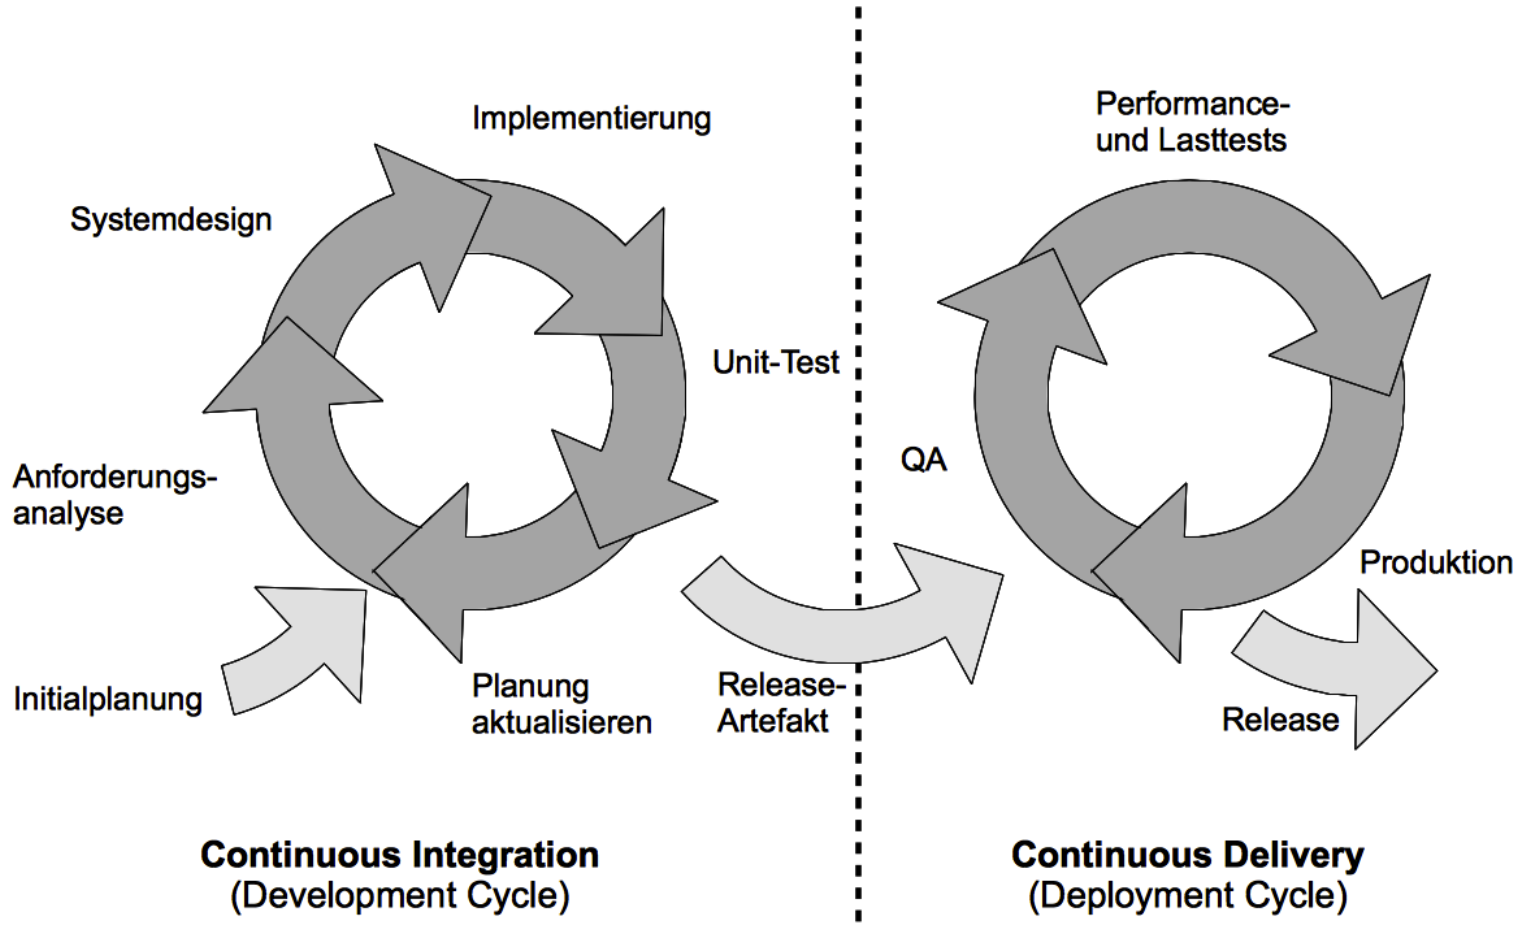
\includegraphics[width=1\textwidth,
		keepaspectratio=true]{bilder/continuous_delivery.png}
\end{frame}

\begin{frame}
\frametitle{Test-Pyramide}
	\center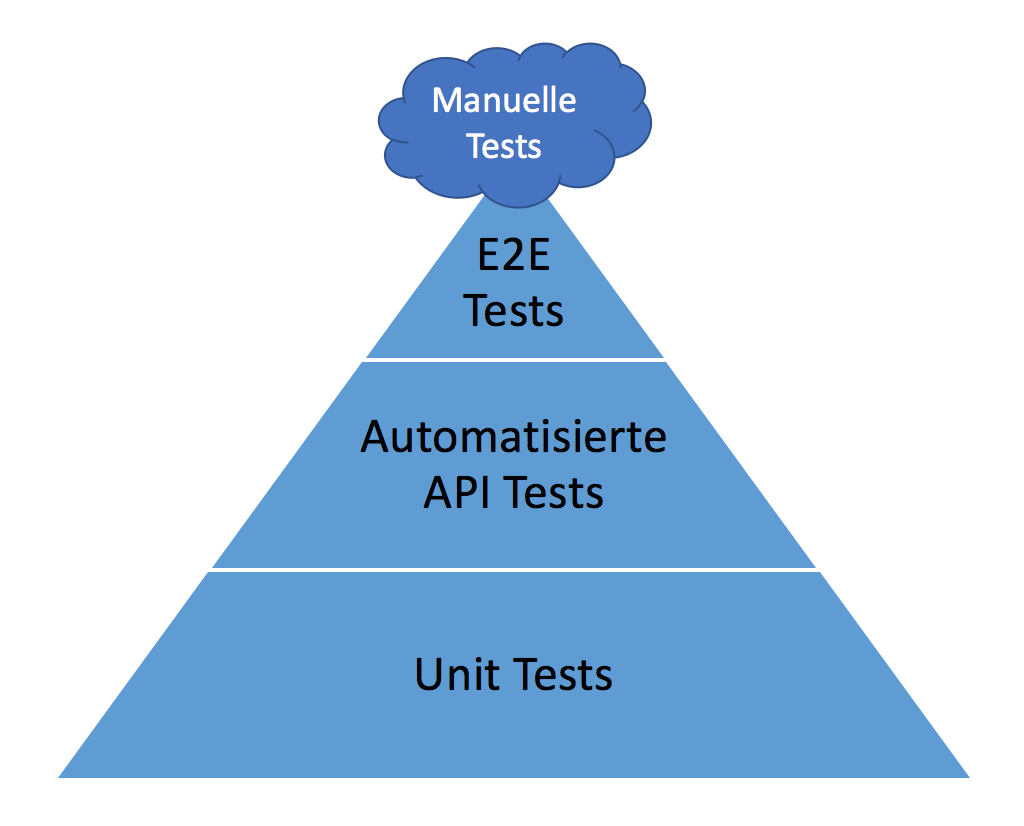
\includegraphics[width=1\textwidth,
		keepaspectratio=true]{bilder/test_pyramide.png}
	\end{frame}

\begin{frame}
\frametitle{Test-Eiswaffel}
	\center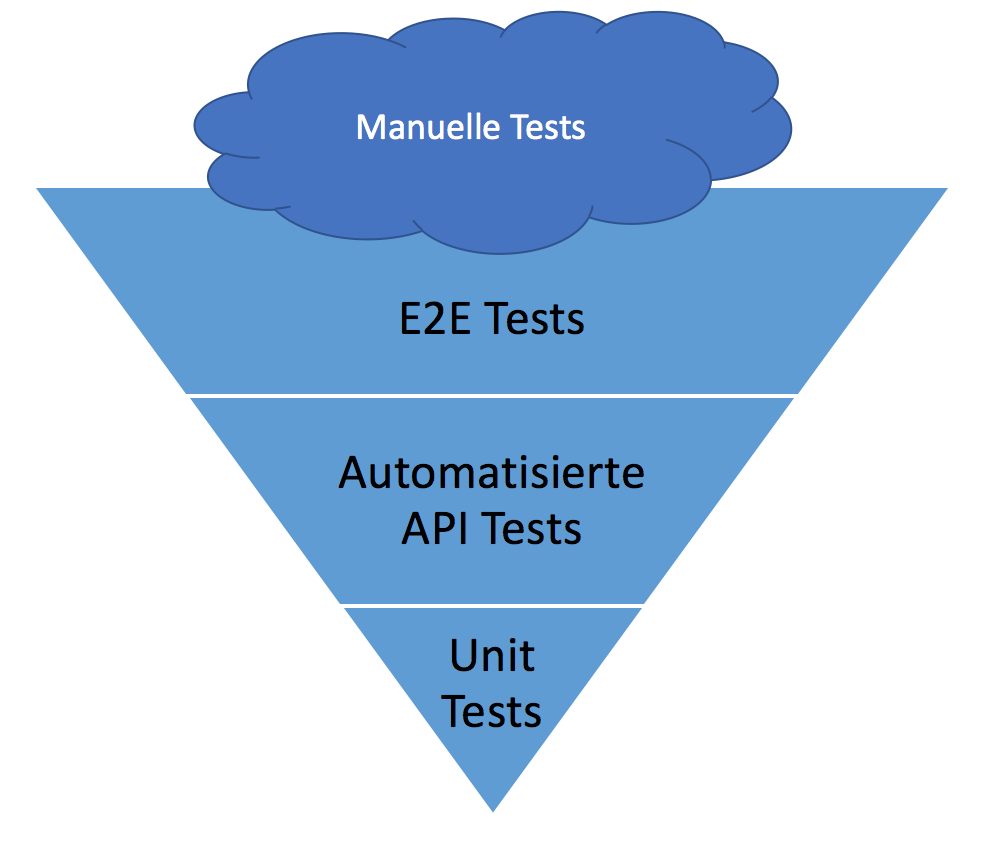
\includegraphics[width=1\textwidth,
		keepaspectratio=true]{bilder/test_eiswaffel.png}
\end{frame}

\begin{frame}
\frametitle{Programmtest}
	\begin{itemize}
		\item Weist fehlerfreiheit des Software-Systems nach
		\item Aufgrund der hohen Komplexität ist Nachweis von Fehlerfreiheit unmöglich
		\item Ziel des Testens ist es daher möglichst viele vorhandene Fehler zu finden
		\item Konkretes Programm wird dazu ausgeführt und mit Werten gefüttert
		\item Ist-Werte werden mit den Soll-Werten aus der Spezifikation verglichen
		\item Bei Abweichung zwischen Ist-Wert und Soll-Wert liegt ein Fehler vor
	\end{itemize}
\end{frame}

\begin{frame}
\frametitle{Programmtest}
	Systematische Tests
	\begin{itemize}
		\item Randbedingungen (z.B. Systemumgebung) ist definiert
		\item Eingaben werden systematisch ausgewählt
		\item Soll-Werte werden vor dem Test festgelegt
		\item Gesamter Test wird dokumentiert
		\item Test und Korrektur finden getrennt statt
	\end{itemize}
	Systematische Tests sind stets reproduzierbar und damit objektiv und wiederholbar.
\end{frame}

\begin{frame}
\frametitle{Programmtest}
	Es können verschiedene Eigenschaften eines Programms getestet werden woraus sich folgende
	Testklassifikation ergibt
	\begin{itemize}
		\item Funktionstest
		\item Last- und Stresstest
		\item Verfügbarkeitstest
		\item Installationstest
		\item Wiederinbetriebnahmetest
	\end{itemize}
	Mindestens Funktions- oder Lasttests sollten systematisch durchgeführt werden.
\end{frame}

\begin{frame}
\frametitle{Programmtest}
	\begin{itemize}
		\item Ein vollständiger Test deckt alle möglichen Eingaben für ein Programm ab
		\item Ist ein vollständiger Test fehlerfrei wurde die Korrektheit des Programms bewiesen
		\item Bereits für einfache Funktion mit ganzahligem Parameter ergibt dies 2\textsuperscript{32} Möglichkeiten
		\item Aus diesem Grund wird Teilmenge getestet und die Eingaben werden geeignet gewählt
	\end{itemize}
\end{frame}

\begin{frame}
\frametitle{Black-Box Test}
	\begin{block}{Black-Box Test}
		Testfälle werden auf Basis der in der Spezifikation geforderten Eigenschaften gewählt.
		Die innere Beschaffenheit des Programms spielt keine Rolle.
	\end{block}
	\begin{itemize}
		\item Testfälle werden aufgestellt sobald die Spezifikation vorliegt
		\item Folgende Verfahren werden zur Bestimmung der Testfälle betrachtet:
			\begin{itemize}
				\item Funktionale Äquivalenzklassenbildung
				\item Grenzwertanalyse
				\item Test spezieller Werte
				\item Zufallstest
			\end{itemize}
	\end{itemize}
\end{frame}

\begin{frame}
\frametitle{Funktionale Äquivalenzklassenbildung}
	\begin{itemize}
		\item Angenommen es existiert eine Menge E = {e1, e2, ..., en} von Eingaben auf die das
					das Programm identisch reagiert
		\item Dann reicht es aus lediglich eine Eingabe dieser Menge zu testen
		\item Wenn die Eingabe fehlerfrei ist kann man von Korrektheit der restlichen Eingaben ausgehen
		\item Eine solche Menge wird als Äquivalenzklasse bezeichnet
		\item Jede Eingabe aus der Äquivalenzklasse ist damit repräsentativ für jede andere Eingabe
					der Äquivalenzklasse
		\item In der Praxis wird häufig nur vermutet das Eingaben Äquivalent, dann wird auch von
					schwacher Äquivalenz gesprochen
	\end{itemize}
\end{frame}

\begin{frame}
\frametitle{Vorgehen bei Äquivalenzklassentest}
	\begin{enumerate}
		\item Menge der Eingaben wird in Äquivalenzklassen zerlegt
		\item Testfälle werden aus Eingaben aus möglichst vielen Äquivalenzklassen zusammengestellt
		\item Ein Testfall sollte höchstens nur eine Eingabe aus einer ungültigen Äquivalenzklasse
					enthalten um die Fehlerbehandlung klar identifizieren zu können
	\end{enumerate}
\end{frame}

\begin{frame}
\frametitle{Grenzwertanalyse}
	\begin{itemize}
		\item Besitzen die Äquivalenzklassen eine natürliche Ordnung werden die Elemente der Klasse
					gewählt die an den Grenzen liegen
		\item Annäherung an die Grenzen kann vom gültigen und vom ungültigen Bereich der Klasse erfolgen
	\end{itemize}
\end{frame}

\begin{frame}
\frametitle{Test spezieller Werte}
	\begin{itemize}
		\item Bei zunehmender Testerfahrung werden Eingaben identifiziert die fehleranfälliger sind
					als andere
		\item Diese Eingaben werden für spätere Testfälle dokumentiert
		\item Beispiele: leere Eingabe, Sonderzeichen
	\end{itemize}
\end{frame}

\begin{frame}
\frametitle{Zufallstest}
	\begin{itemize}
		\item Testfälle werden zufällig generiert
		\item Datentypen und Struktur der Eingaben müssen bei Generierung berücksichtigt werden
		\item Ist ein ergänzendes Verfahren
		\item Deckt auch nicht naheliegene Eingaben ab
	\end{itemize}
\end{frame}

\begin{frame}
\frametitle{White-Box Test}
	\begin{block}{White-Box Test}
		Der Programmcode ist sichtbar. Es wird ein Strukturtest vorgenommen. Dabei wird die
		überdeckung des Codes durch die Testfälle analysiert. Das Ziel ist es eine vorgegebene
		Überdeckungsrate zu erreichen.
	\end{block}
	\begin{itemize}
		\item Um die Überdeckungsrate bestimmen zu können muss das Programm mit zusätzlichen
					Anweisungen für die Messung instrumentiert werden
		\item Dadurch kann z.B. gezählt werden wie häufig eine Programmzeile ausgeführt wurde
		\item Es werden verschiedene Überdeckungskriterien unterschieden
					\begin{itemize}
						\item Anweisungsüberdeckung
						\item Zweigüberdeckung
						\item Bedingungsüberdeckung
					\end{itemize}
	\end{itemize}
\end{frame}

\subsection{Messen/Bewerten}
\begin{frame}
\frametitle{Messen und Bewerten}
\huge Messen und Bewerten
\end{frame}

\begin{frame}
\frametitle{Projekt-Controlling - Fertigstellungsgrad}

\end{frame}

\begin{frame}
\frametitle{Projekt-Controlling - EVA}

\end{frame}

\begin{frame}
\frametitle{Software-Metriken}

\end{frame}


%%\part{Entwurfsprinzipien}

%----------------------------------------------------------------------------
\section{Requirements Engineering}
\begin{frame}[fragile]
	\frametitle{Requirements Engineering}
\huge Requirements Engineering
\end{frame}


%%\part{advanced_oo}

%----------------------------------------------------------------------------
\section{SW Architektur}
\begin{frame}[fragile]
	\frametitle{Software Architektur}
\huge Software Architektur
\end{frame}


%%\part{Grundlagen}

%----------------------------------------------------------------------------
\section{Konfigurations - Management}
\begin{frame}[fragile]
	\frametitle{Konfigurationsmanagement}
\huge Konfigurationsmanagement
\end{frame}


\end{document}
